
% This LaTeX was auto-generated from MATLAB code.
% To make changes, update the MATLAB code and republish this document.

\documentclass{article}
\usepackage{graphicx}
\usepackage{color}

\sloppy
\definecolor{lightgray}{gray}{0.5}
\setlength{\parindent}{0pt}

\begin{document}

    
    \begin{verbatim}
function firstTask
h=0.1;%стъпка
x=0:h:1*10;
n=length(x);%итерации
y(1,1)=0; y(2,1) = 0.16;%начални условия
for i=1:(n-1)
    k1=h*system (x(i), y(1:2,i));
    k2=h*system (x(i) + h/2, y(1:2, i) + h*k1/2);
    k3=h*system (x (i) + h/2, y(1:2, i) + h*k2/2);
    k4=h*system (x(i) + h, y(1:2, i) +h*k3);
    y(1:2, i+1)=y(1:2, i) + (h*(k1+2*k2+2*k3+k4))/6;
end
figure (1), plot (x,y (1, :),x,y(2,:));
legend('y_1', 'y_2','Location', 'best');
title('Решение на системата по Рунге-Кута');
end

function f = system (x, y)
    f(1,1)=y(2);
    f(2,1)=0.05*x*y(2)-x^2*y(1);
end
\end{verbatim}

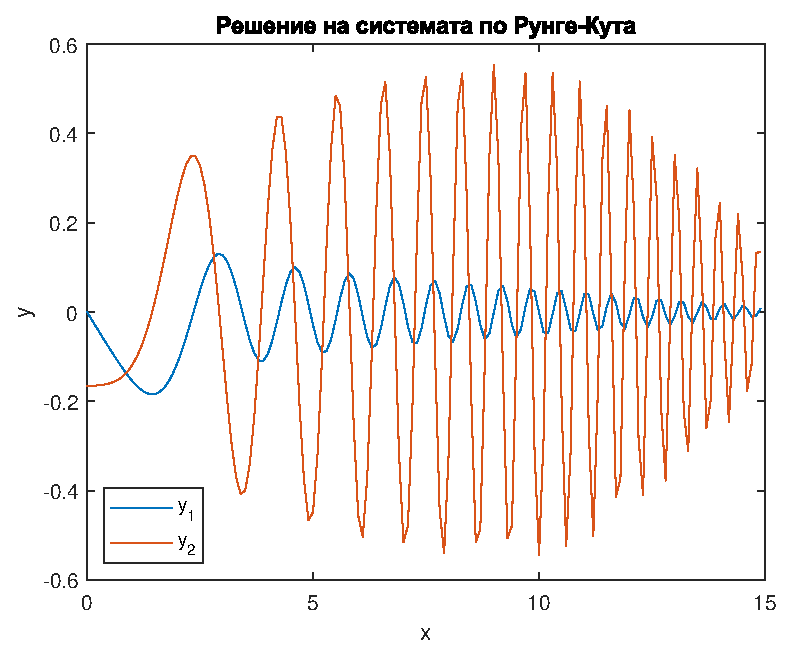
\includegraphics [width=4in]{firstTask_01.eps}



\end{document}

